%!TEX root =  GDELT_GA_Search_UsersManual.tex

\chapter{Prediction Methods} \label{chap:PredictionMethods}

\section{Definitions}

\textbf{Predictions} are created from known periods of time and are used on unknown periods of time. 
As such, making predictions requires splitting time in two places. 

\begin{enumerate} 
  \item The first split occurs \emph{before} or \emph{after} the point of transition from known to unknown.  The \textit{before} period is called \textbf{training} and the \textit{after} period is called \textbf{testing}. The \textit{point of transition} from before to after is called \textbf{time zero}. 
  \item The second split occurs between the the GDELT data (i.e., independent variables) and the target time-series (social media) event counts (i.e., dependent variables). The GDELT data belong to \textbf{X} and social media event counts belong to \textbf{Y}.\footnote{This vocabulary is based on graphs in which the values of the independent variable are placed on the (horizontal) x-axis and the values of the dependent variable are placed on the (vertical) y-axis.} 
\end{enumerate}

\par Making these two splits results in a total of four periods:

\begin{itemize} 
\item \textbf{X-Train}	- GDELT training
\item \textbf{Y-Train}	- Social media event counts training
\item \textbf{X-Test} - GDELT testing
\item \textbf{Y-Test} - Social media event counts testing
\end{itemize}

\begin{figure}
[htbp] 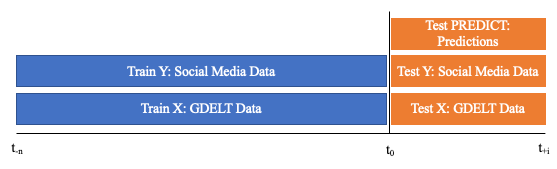
\includegraphics[width=\columnwidth]{PredictGraph.png}
\caption{Conceptual View of the Prediction Process} 
\label{PredictGraphFigure} 
\end{figure}

\par In the canonical case, %of what? "in the canonical case of prediction, predict using the following", maybe
 a prediction is made using the following: X-Train is compared to Y-Train to establish the relationship between them (e.g., a linear correlation). Then, X-Test is used to create a time series for the testing period; this is termed the Y-Predict. It is then possible to score the performance of the prediction by comparing Y-Predict with the Y-Test values, which contain the `correct' answer.

\par This can represent this as a function:

\begin{equation}
  Y_{predict} = f(Y_{Train},X_{Train},X_{Test})
\end{equation}

\par or

\begin{equation}
  y_{t0}, y_{t1}, y_{t2}, ... y_{ti} = f([y_{t-n}, ...y_{t-2}, y_{t-1}],[x_{t-n}, ...x_{t-2}, x_{t-1}],[x_{t0}, x_{t1}, x_{t2}, ... x_{ti}])
\end{equation}


\par While this is a canonical case, %of prediction?
 it is not the only case. For example, some predictions may need to be made without using X-Test. A true forecast into an unknown future, such as attempting to predict social media events days or weeks in advance, would be done without the values in X-Test, because the GDELT data in X-Test would also be unknown. In equation form:

\begin{equation}
  Y_{predict} = f(Y_{Train},X_{Train})
\end{equation}

\par Typically, the training period is longer than the prediction period. This is especially so in the second form, as predicting into the unknown without the X-Test values available is difficult.

\par The units for the time series values are usually `days', so that the series values are `events per day'. However, this can be changed and the series can be created for any unit of time (e.g., 4 hours). The limit is the resolution of the data. In GDELT, the event data are identified by the `day' field, which is a calendar date with no meaningful time stamp; however, the field \textit{dateadded} field can be used, and this has a 15-minute resolution. The dateadded field can also be more appropriate if what is being examined is the relationship between the dependent variable (e.g., social media data) and the appearance of an event in the news rather than the event itself---that is, when the event was being discussed in the news and not when the event actually happened.

\section{Prediction Methods}
\subsection{Raw}
\subsection{Base Values}
\section{Replay}
 A category of predictions known as \textbf{replay} has a simple idea: take values from the training period and repeat them in the testing period.
\par Variations on this theme are possible. For example, given the need to predict 8 days into the future, one could simply replay the 8 days immediately prior to $t_0$. Alternatively, one could align the days being replayed by day of the week, to catch weekly cycles of high and low activity.

\subsection{Linear Regression}
\subsubsection{Linear Regression Weighted}

\section{Long Short-Term Memory}


\section{Elastic Net}
\section{Gradient Boost}
\section{Lasso}
\section{Adding Prediction Methods}
\subsection{Java}

\par Creating new prediction methods in Java is straightforward: All prediction classes must implement 
\subsection{Python}



